\documentclass[a4paper,12pt]{article}
\usepackage{amsmath, amssymb}
\usepackage{xcolor}
\usepackage[most]{tcolorbox}
\usepackage{multicol}
\usepackage{geometry}
\usepackage{enumitem}
\graphicspath{ {../Images/} }
\hyphenpenalty=100000

\geometry{left=1.5cm, right=1.5cm, top=2cm, bottom=2cm}

\tcbuselibrary{theorems}

\definecolor{PurpleEx}{HTML}{5d478b}
\definecolor{GrayEx}{HTML}{f2f2f2}
\definecolor{GrayBG}{HTML}{d9d9d9}
\definecolor{BlackSav}{HTML}{000000}

\title{
\centering
\tcbset{colframe=BlackSav,colback=GrayBG}
\tcbox[tikznode]{
Chapitre 5 \\Dérivation et applications
}
}
\usepackage{tikz}
\author{}
\date{}

\newtcbtheorem
  []% init options
  {exercice}% name
  {Exercice}% title
  {%
    colback=GrayEx,
    colframe=PurpleEx,
    fonttitle=\bfseries,
    breakable=true
  }% options
  {ex}% prefix

\begin{document}

\maketitle

\begin{multicols}{2}
% Exercice 1
\begin{exercice}[title=Exercice 1 $\quad \star \quad$ { [Représenter] }]{}{}
On donne le tableau de signes de la dérivée $f'$ d'une fonction $f$ définie et dérivable sur $\mathbb{R}$.
\begin{center}
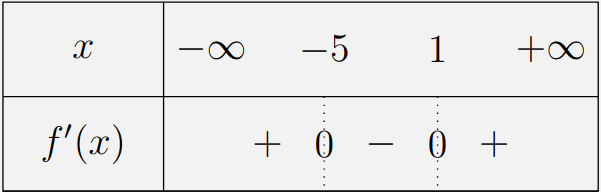
\includegraphics[width=0.8\linewidth]{swappy-20241230_104216.png}
\end{center}
Déterminer les variations de la fonction $f$.
\end{exercice}

% Exercice 2
\begin{exercice}[title=Exercice 2 $\quad \star \quad$ { [Représenter] }]{}{}
On considère la fonction $f$ définie sur $\mathbb{R}$ dont la courbe est représentée ci-dessous.
\begin{center}
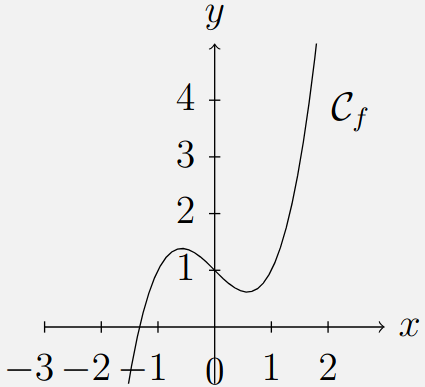
\includegraphics[height=0.7\linewidth]{swappy-20241230_104240.png}
\end{center}
Parmi les trois représentations graphiques ci-contre, laquelle est susceptible de représenter la fonction $f'$, fonction dérivée de la fonction $f$ sur $\mathbb{R}$ ?
\pagebreak
\begin{enumerate}
  \item
  ~\\\begin{center}
    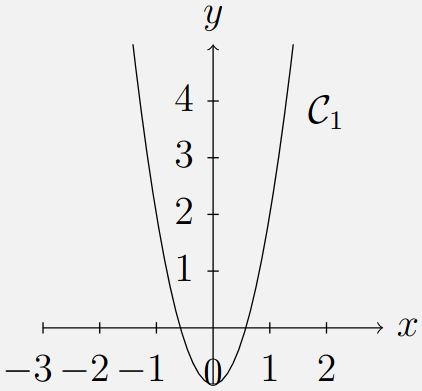
\includegraphics[height=0.7\linewidth]{swappy-20241230_104259.png}
    \end{center}
  \item
  ~\\\begin{center}
    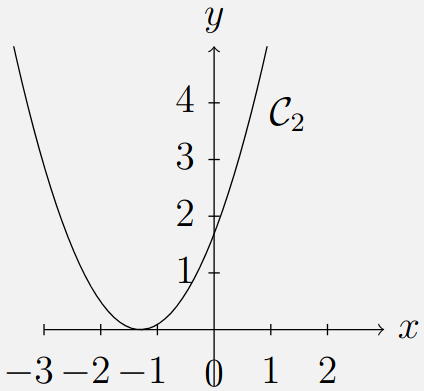
\includegraphics[height=0.7\linewidth]{swappy-20241230_104325.png}
    \end{center}
  \item 
  ~\\\begin{center}
    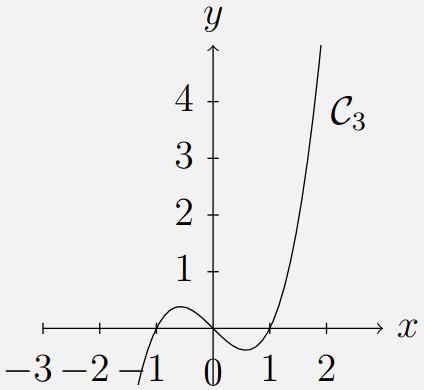
\includegraphics[height=0.7\linewidth]{swappy-20241230_104346.png}
    \end{center}
\end{enumerate}
\end{exercice}

% Exercice 3
\begin{exercice}[title=Exercice 3 $\quad \star \quad$ { [Représenter] }]{}{}
Chaque courbe est la représentation graphique de la fonction dérivée $f'$. Dans chaque cas, tracer une courbe susceptible de représenter $f$.  
Remarque : les trois premières fonctions sont définies et dérivables sur $\mathbb{R}$ alors que la quatrième est définie et dérivable sur $\mathbb{R}^*$.
\begin{enumerate}
  \item
  ~\\\begin{center}
    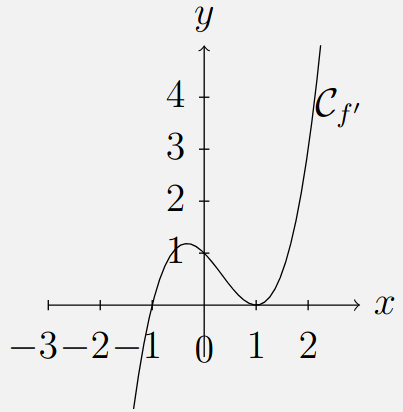
\includegraphics[height=0.55\linewidth]{swappy-20241230_104402.png}
    \end{center}
  \item
  ~\\\begin{center}
    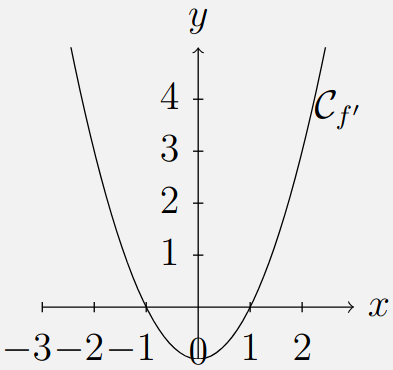
\includegraphics[height=0.5\linewidth]{swappy-20241230_104414.png}
    \end{center}
  \item
  ~\\\begin{center}
    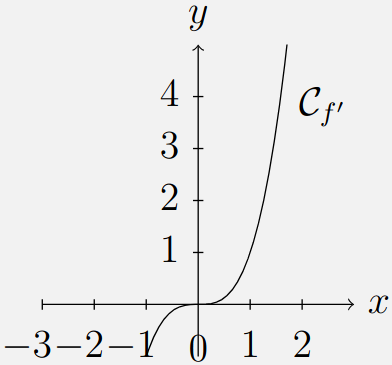
\includegraphics[height=0.5\linewidth]{swappy-20241230_104431.png}
    \end{center}
  \item
  ~\\\begin{center}
    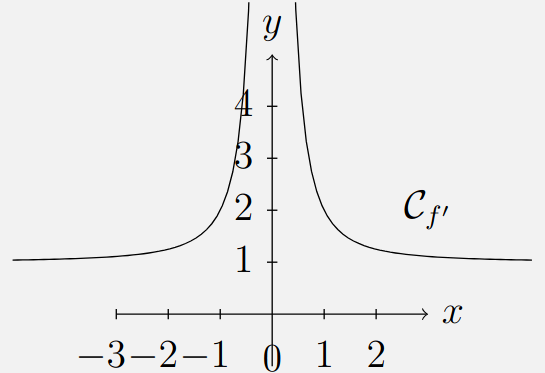
\includegraphics[height=0.5\linewidth]{swappy-20241230_104450.png}
    \end{center}
\end{enumerate}
\end{exercice}

% Exercice 4
\begin{exercice}[title=Exercice 4 $\quad \star\star \quad$ { [Raisonner] }]{}{}
Soit $f$ une fonction définie et dérivable sur $\mathbb{R}$.
\begin{enumerate}
    \item La propriété suivante est-elle vraie ou fausse ? « Si $f'(x) > 0$ pour tout $x \in \mathbb{R}$, alors $f$ est strictement croissante sur $\mathbb{R}$ ».
    \item Énoncer la réciproque de cette propriété. Est-elle vraie ou fausse ?
\end{enumerate}
\end{exercice}

% Exercice 5
\begin{exercice}[title=Exercice 5 $\quad \star\star \quad$ { [Raisonner] }]{}{}
Soit $f$ une fonction définie et dérivable sur $\mathbb{R}$.
\begin{enumerate}
    \item La propriété suivante est-elle vraie ou fausse ? « Si $f$ admet un extremum local en $x = 2$, alors $f'(2) = 0$ ».
    \item Énoncer la réciproque de cette propriété. Est-elle vraie ou fausse ?
\end{enumerate}
\end{exercice}

% Exercice 6
\begin{exercice}[title=Exercice 6 $\quad \star\star \quad$ { [Raisonner] }]{}{}
La propriété suivante est-elle vraie ou fausse ? « Si pour tout $x \in \mathbb{R}$, $f(x) = 3x^2 + 2$, alors pour tout $x \in \mathbb{R}$, $f'(x) = 6x$ ».  
Énoncer la réciproque de cette propriété. Est-elle vraie ou fausse ?
\end{exercice}

% Exercice 7
\begin{exercice}[title=Exercice 7 $\quad \star \quad$ { [Calculer] }]{}{}
Étudier les variations de la fonction $f$ définie sur $\mathbb{R}$ par $f(x) = 5x^2 - 3x + 2$.
\end{exercice}

% Exercice 8
\begin{exercice}[title=Exercice 8 $\quad \star \quad$ { [Calculer] }]{}{}
Étudier les variations de la fonction $f$ définie sur $\mathbb{R}$ par $f(x) = \dfrac{1}{3}x^2 - \dfrac{5}{2}x + 1$.
\end{exercice}

% Exercice 9
\begin{exercice}[title=Exercice 9 $\quad \star \quad$ { [Calculer] }]{}{}
Étudier les variations de la fonction $f$ définie sur $\mathbb{R}$ par $f(x) = x^3 + 5x^2 - 3x + 1$.
\end{exercice}
    
% Exercice 10
\begin{exercice}[title=Exercice 10 $\quad \star \quad$ { [Calculer] }]{}{}
Étudier les variations de la fonction $f$ définie sur $\mathbb{R}$ par $f(x) = 2x^3 - x^2 + 2x - 5$.
\end{exercice}

% Exercice 11
\begin{exercice}[title=Exercice 11 $\quad \star \quad$ { [Calculer] }]{}{}
Étudier les variations de la fonction $f$ définie sur $\mathbb{R}$ par $f(x) = x^4 + 5x^2 - 4$.
\end{exercice}

% Exercice 12
\begin{exercice}[title=Exercice 12 $\quad \star \quad$ { [Calculer] }]{}{}
Étudier les variations de la fonction $f$ définie sur $\mathbb{R} \setminus \{7\}$ par $f(x) = \dfrac{x+1}{x-7}$.
\end{exercice}

% Exercice 13
\begin{exercice}[title=Exercice 13 $\quad \star \quad$ { [Calculer] }]{}{}
Étudier les variations de la fonction $f$ définie sur $\mathbb{R}$ par $f(x) = \dfrac{x}{x^2 + 1}$.
\end{exercice}

% Exercice 14
\begin{exercice}[title=Exercice 14 $\quad \star \quad$ { [Calculer] }]{}{}
Étudier les variations de la fonction $f$ définie sur $\mathbb{R} \setminus \{0\}$ par $f(x) = x - 4 + \dfrac{2}{x}$.
\end{exercice}

% Exercice 15
\begin{exercice}[title=Exercice 15 $\quad \star \quad$ { [Calculer] }]{}{}
Étudier les variations de la fonction $f$ définie sur $\mathbb{R}$ par $f(x) = \dfrac{2x^2 + 12x}{x^2 + 4}$.
\end{exercice}

% Exercice 16
\begin{exercice}[title=Exercice 16 $\quad \star \quad$ { [Calculer] }]{}{}
Étudier les variations de la fonction $f$ définie sur $[\dfrac{4}{3}; +\infty[$ par $f(x) = \sqrt{3x-4}$.
\end{exercice}

% Exercice 17
\begin{exercice}[title=Exercice 17 $\quad \star \star \star \quad$ { [Calculer] }]{}{}
Étudier les variations de la fonction $f$ définie sur $\mathbb{R}$ par $$f(x) = \dfrac{x^4}{2} - \dfrac{2x^3}{3} + 2x^2 - 4x + 5.$$
\end{exercice}

% Exercice 18
\begin{exercice}[title=Exercice 18 $\quad \star \star \quad$ { [Calculer] }]{}{}
Étudier les variations de la fonction $f$ définie sur $]-4; +\infty[$ par $f(x) = \dfrac{x^3 - 2}{x + 4}$.
\end{exercice}

\vfill

% Exercice 19
\begin{exercice}[title=Exercice 19 $\quad \star \star \quad$ { [Calculer] }]{}{}
On considère la suite définie par $$u_n = n^4 - 2n^3 - 5n^2 - 1$$ pour $n \geq 0$. À l'aide de calculs, déterminer les variations de $(u_n)_{n \in \mathbb{N}}$.
\end{exercice}

\vfill

% Exercice 20
\begin{exercice}[title=Exercice 20 $\quad \star \star \quad$ { [Calculer] }]{}{}
Soit $f(x) = x^2 - 3x + 1$. Pour $x \in [1; 5]$, déterminer un encadrement de $f(x)$.
\end{exercice}

\vfill

% Exercice 21
\begin{exercice}[title=Exercice 21 $\quad \star \star \quad$ { [Calculer, Raisonner] }]{}{}
Soit $f(x) = 8x^4 - 8x^2 + 1$. Montrer que :
\[
-1 \leq x \leq 1 \iff -1 \leq f(x) \leq 1.
\]
\end{exercice}

\vfill

% Exercice 22
\begin{exercice}[title=Exercice 22 $\quad \star \star \quad$ { [Représenter] }]{}{}
On considère les fonctions $f$ et $g$ définies sur $\mathbb{R}$ par $f(x) = x^4$ et $g(x) = 2x^3 - 2x^2 - 10$. Déterminer la position relative de $C_f$ et de $C_g$.
\end{exercice}

\vfill

% Exercice 23
\begin{exercice}[title=Exercice 23 $\quad \star \star \star \quad$ { [Calculer, Représenter] }]{}{}
On considère les fonctions $f$ et $g$ définies sur $\mathbb{R}$ par $f(x) = x^3 - 3x$ et $g(x) = x - \dfrac{4}{x}$. Déterminer la position relative de $C_f$ et $C_g$.
\end{exercice}


\vfill

\newpage

% Exercice 24
\begin{exercice}[title=Exercice 24 $\quad \star \star \star \quad$ { [Calculer, Représenter] }]{}{}
Soit la fonction définie sur $\mathbb{R} \setminus \{1\}$ par 
\[
f(x) = \dfrac{-2x^2 + 3x - 2}{x - 1}.
\]
\begin{enumerate}
  \item Déterminer les variations de $f$.
  \item Montrer que pour tout $x \in \mathbb{R} \setminus \{1\}$, $f(x) = -2x + 1 - \dfrac{1}{x-1}$.
  \item On note $d$ la droite d’équation $y = -2x + 1$.
  \begin{enumerate}
    \item Déterminer la limite suivante :
    \[
    \lim_{x \to +\infty} \left( f(x) - (-2x + 1) \right).
    \]
    \item Interpréter graphiquement ?
  \end{enumerate}
  \item Étudier la position relative de $C_f$ par rapport à $d$.
\end{enumerate}
\end{exercice}

% Exercice 25
\begin{exercice}[title=Exercice 25 $\quad \star \star \quad$ { [Modéliser, Calculer] }]{}{}
On considère un carré $ABCD$ de côté $AB = 1$. $EFGH$ est un carré tel que :
\begin{itemize}
  \item Les points $E$, $F$, $G$, $H$ appartiennent respectivement aux côtés $[AB]$, $[BC]$, $[CD]$ et $[AD]$.
  \item $AE = BF = CG = DH = x$ avec $0 \leq x \leq 1$.
\end{itemize}
\begin{center}
  
\includegraphics[width=0.6\linewidth]{swappy-20241230_104523.png}
\end{center}
Déterminer la valeur de $x$ pour laquelle l'aire du carré $EFGH$ est minimale.
\end{exercice}

% Exercice 26
\begin{exercice}[title=Exercice 26 $\quad \star \star \quad$ { [Modéliser, Calculer] }]{}{}
On dispose d’une feuille A4 cartonnée $(210 \times 297 \, \text{mm})$ avec laquelle on souhaite fabriquer une boîte. On découpe la feuille au niveau des pointillés et on relève les rabats afin d’obtenir une boîte sans couvercle. On note $x$ la hauteur de la boîte en mm et $\mathcal{V}(x)$ son volume en mm$^3$.
\begin{center}
  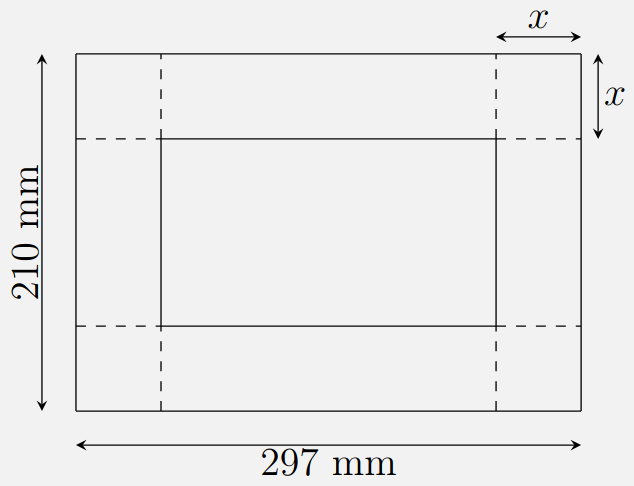
\includegraphics[width=0.9\linewidth]{swappy-20241230_104609.png}
\end{center}
Déterminer la valeur de $x$ telle que le volume de la boîte soit maximal.
\end{exercice}

% Exercice 27
\begin{exercice}[title=Exercice 27 $\quad \star \star \quad$ { [Modéliser, Calculer] }]{}{}
On souhaite fabriquer une casserole de $2$ litres. Quelles doivent être les dimensions de la casserole afin que la quantité de métal utilisé soit minimale ?
\end{exercice}

% Exercice 28
\begin{exercice}[title=Exercice 28 $\quad \star \star \quad$ { [Modéliser, Calculer] }]{}{}
Un éditeur doit produire un livre avec les contraintes suivantes : sur chaque page, le texte imprimé doit être contenu dans un rectangle de $300 \, \text{cm}^2$ ; les marges à gauche et à droite doivent mesurer $1.5 \, \text{cm}$ et les marges en haut et en bas doivent mesurer $2 \, \text{cm}$. Quelles doivent être les dimensions d’une page pour que la consommation de papier soit minimale ?
\end{exercice}

% Exercice 29
\begin{exercice}[title=Exercice 29 $\quad \star \star \star \quad$ { [Chercher, Modéliser, Calculer] }]{}{}
On souhaite construire une autoroute entre deux villes $A$ et $D$. La partie $[AC]$ existe déjà, mais doit subir une rénovation entre $A$ et $B$ qui coûte $2$ millions d’euros par kilomètre pour être utilisable. Le tronçon $[BD]$ est à construire neuf et coûte $4$ millions d’euros par km. Où doit-on placer le point $B$ sur le segment $[AC]$ afin que le coût de construction de l’autoroute soit minimal ?
\begin{center}
  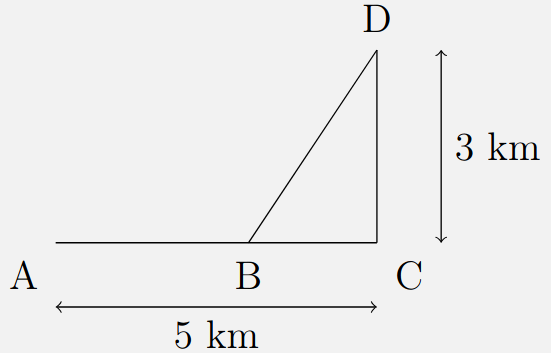
\includegraphics[width=0.7\linewidth]{swappy-20241230_104633.png}
\end{center}
\end{exercice}

% Exercice 30
\begin{exercice}[title=Exercice 30 $\quad \star \star \star \quad$ { [Chercher, Modéliser, Calculer] }]{}{}
Dans un disque en carton de rayon $10 \, \text{cm}$, on découpe un secteur d’angle $\alpha$ (en radians). Avec ce secteur, on souhaite fabriquer un cône de révolution.
\begin{center}
  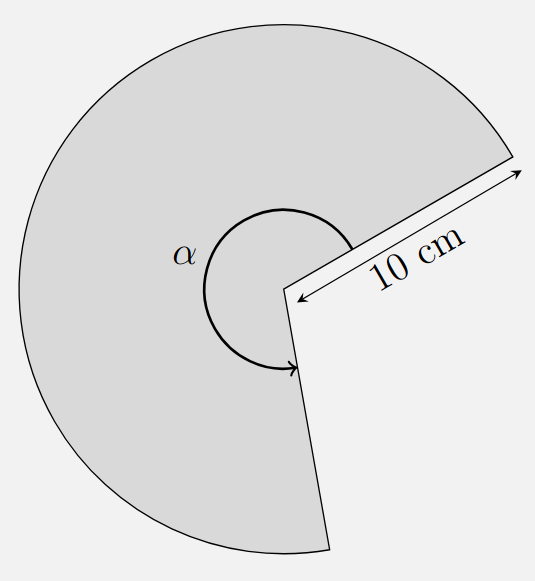
\includegraphics[width=0.8\linewidth]{swappy-20241230_104712.png}
\end{center}
Quelle doit être la valeur de $\alpha$ pour que le volume du cône soit maximal ?
\end{exercice}

% Exercice 31
\begin{exercice}[title=Exercice 31 $\quad \star \star \star \quad$ { [Chercher, Modéliser, Calculer] }]{}{}
Démontrer que parmi les losanges d'aire $S$ donnée, le carré est celui dont le périmètre est minimal.
\end{exercice}

\vfill

% Exercice 32
\begin{exercice}[title=Exercice 32 $\quad \star \star \star \quad$ { [Chercher, Modéliser, Calculer] }]{}{}
$ABC$ est un triangle quelconque, $M$ un point de $[BC]$ à partir duquel on construit le parallélogramme $MQAP$ comme ici-dessous.
\begin{center}
  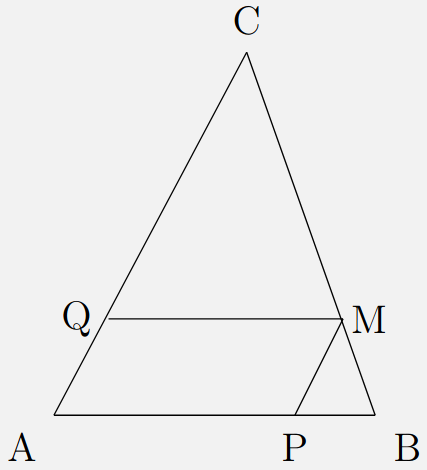
\includegraphics[width=0.6\linewidth]{swappy-20241230_104649.png}
\end{center}
Comment choisir $M$ de sorte que l'aire de ce parallélogramme soit maximale ?
\end{exercice}
\vfill

\newpage

% Exercice 33
\begin{exercice}[title=Exercice 33 $\quad \star \star \quad$ { [Calculer, Modéliser] }]{}{}
Le chikungunya est une maladie virale transmise d’un être humain à l’autre par les piqûres de moustiques femelles infectées.

Un test a été mis au point pour le dépistage de ce virus. Le laboratoire fabriquant ce test fournit les caractéristiques suivantes :
\begin{itemize}[noitemsep, topsep=0pt]
    \item La probabilité qu’une personne atteinte par le virus ait un test positif est de $0,98$.
    \item La probabilité qu’une personne non atteinte par le virus ait un test positif est de $0,01$.
\end{itemize}

On procède à un test de dépistage systématique dans une population « cible ». Un individu est choisi au hasard dans cette population. On appelle :
\begin{itemize}[noitemsep, topsep=0pt]
    \item $M$ l’événement : « L’individu choisi est atteint du chikungunya ».
    \item $T$ l’événement : « Le test de l’individu choisi est positif ».
\end{itemize}

On notera $\overline{M}$ (respectivement $\overline{T}$) l’événement contraire de l’événement $M$ (respectivement $T$).

On note $p \ (0 \leq p \leq 1)$ la proportion de personnes atteintes par la maladie dans la population cible.
\begin{enumerate}
  \item \begin{enumerate}
    \item Représenter la situation par un arbre de probabilités.
    \item Exprimer $P(M \cap T)$, $P(\overline{M} \cap T)$ puis $P(T)$ en fonction de $p$.
  \end{enumerate}
  \item \begin{enumerate}
    \item Démontrer que la probabilité de $M$ sachant $T$ est donnée par la fonction $f$ définie sur $[0; 1]$ par :
    \[
    f(p) = \dfrac{98p}{97p + 1}.
    \]
    \item Étudier les variations de la fonction $f$.
  \end{enumerate}
  \item Considérant que le test est fiable lorsque la probabilité qu’une personne ayant un test positif soit réellement atteinte du chikungunya est supérieure à $0,95$, à partir de quelle proportion $p$ de malades dans la population le test est-il fiable ?
\end{enumerate}
\end{exercice}

\vfill

% Exercice 34
\begin{exercice}[title=Exercice 34 $\quad \star \star \star \quad$ { [Calculer, Modéliser, Chercher] }]{}{}
On considère un nombre réel $x$. Une urne contient $50$ jetons de couleurs bleue, rouge ou jaune. $10\%$ des jetons sont bleus, il y a trois fois plus de jetons jaunes que de jetons bleus. 

Un joueur tire un jeton au hasard :
\begin{itemize}[noitemsep, topsep=0pt]
    \item S’il est rouge, il gagne $x$ euros ;
    \item S’il est jaune, il gagne $x^2$ euros ;
    \item S’il est bleu, il perd $x^3$ euros.
\end{itemize}

Quelle doit être la valeur de $x$ pour que le gain moyen réalisé sur un grand nombre de tirages soit maximal ?
\end{exercice}

\vfill

% Exercice 35
\begin{exercice}[title=Exercice 35 $\quad \star \star \star \quad$ { [Calculer, Modéliser, Chercher] }]{}{}
Une urne contient $3$ boules rouges, $4$ boules bleues et $n$ boules vertes. Les boules sont indiscernables au toucher. On tire successivement et avec remise deux boules de l’urne. On note $X$ le nombre de couleurs apparues. Quelle est la valeur de $n$ pour laquelle l’espérance de $X$ est maximale ?
\end{exercice}

\vfill

\newpage

% Exercice 36
\begin{exercice}[title=Exercice 36 $\quad \star \star \quad$ { [Modéliser, Calculer, Raisonner] }]{}{}
Un automobiliste parcourt une distance de $240$ km sur une autoroute où la vitesse est limitée à $130 \ \text{km.h}^{-1}$. La distance parcourue en fonction du temps (en heures) est représentée ci-dessous.
\begin{center}
  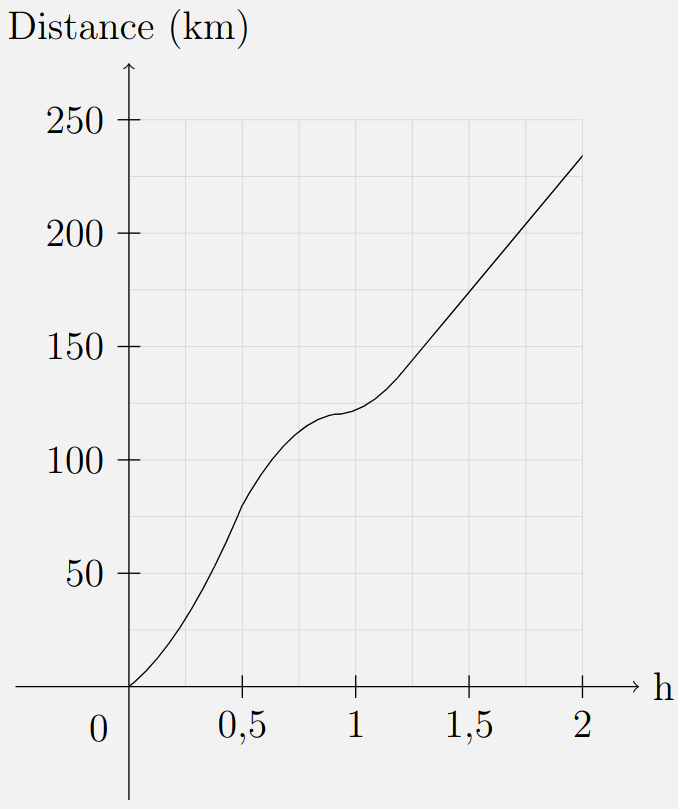
\includegraphics[width=0.8\linewidth]{swappy-20241230_104742.png}
\end{center}
\begin{enumerate}
    \item Que pensez-vous du raisonnement suivant ? « L’automobiliste a parcouru les $240$ km en $2$ h, soit une moyenne de $130 \ \text{km.h}^{-1}$, il ne recevra donc pas d’amende ».
    \item Déterminer graphiquement, et le plus précisément possible, la vitesse de la voiture à l’instant $t = 1$ h.
    \item De manière générale, si la fonction $f$ désigne la distance parcourue par la voiture en fonction du temps, comment calcule-t-on la vitesse au temps $t$ ?
    \item Déterminer sa vitesse maximale au cours du trajet. L’automobiliste a-t-il dépassé la vitesse autorisée ?
\end{enumerate}
\end{exercice}

\vspace{3em}

% Exercice 37
\begin{exercice}[title=Exercice 37 $\quad \star \star \quad$ { [Modéliser, Calculer, Représenter] }]{}{}
L'objectif de cet exercice est d'étudier la vitesse de propagation d'une maladie. Le nombre de malades en fonction du temps $t$, exprimé en jours, peut-être modélisé par la fonction $f$, définie et dérivable sur l'intervalle $[0; 30]$ par $f(t) = -t^3 + 30t^2$. La courbe représentative de $f$ est donnée ci-dessous.
\begin{center}
  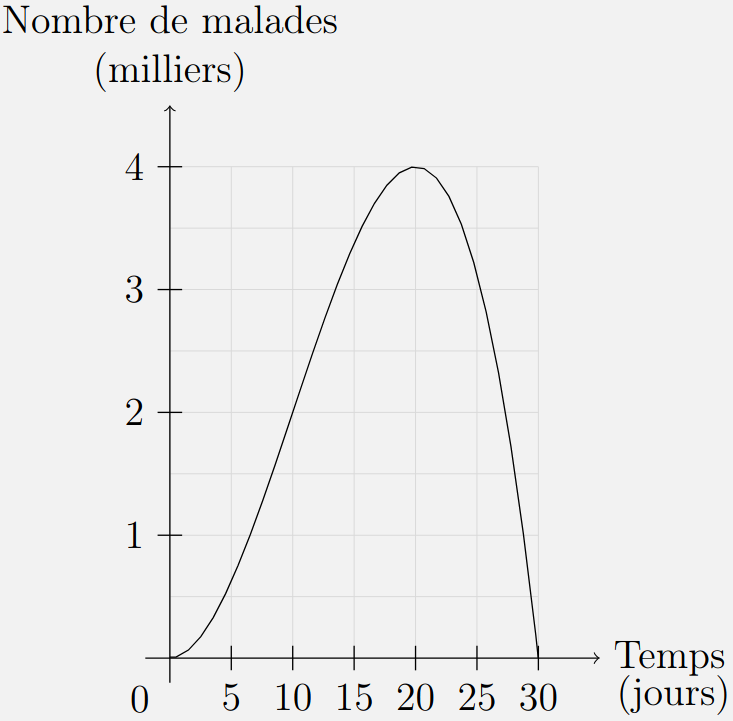
\includegraphics[width=0.9\linewidth]{swappy-20241230_104801.png}
\end{center}
On note $v(t)$ la vitesse de propagation de la maladie au temps $t$ c’est-à-dire le nombre de malades supplémentaires par jour (si le nombre de malades diminue, la vitesse devient alors négative).
\begin{enumerate}
    \item Déterminer la vitesse moyenne de propagation entre le déclenchement de la maladie ($0^\text{ème}$ jour) et le $10^\text{ème}$ jour.
    \item Déterminer graphiquement :
    \begin{enumerate}
        \item Quel est le jour où le nombre de malades était maximum ? Quelle est alors la vitesse de propagation de la maladie ce jour-là ?
        \item À partir de quel jour la vitesse de propagation de la maladie diminue-t-elle ?
    \end{enumerate}
    \item Exprimer la vitesse de propagation $v(t)$. Étudier les variations de $v$ et retrouver l'ensemble des résultats de la question 2.
\end{enumerate}
\end{exercice}

% Exercice 38
\begin{exercice}[title=Exercice 38 $\quad \star \star \quad$ { [Modéliser, Calculer, Représenter] }]{}{}
L'eau oxygénée $H_2O_2$ est utilisée de diverses manières, par les médecins comme antiseptique, par les coiffeurs pour décolorer les cheveux ou encore par l'industrie pour blanchir le papier par exemple. L'eau oxygénée se décompose naturellement pour former de l'eau $H_2O$ et de l'oxygène $O_2$. 

On réalise deux expériences : une première en plaçant de l'eau oxygénée seule dans un récipient fermé et une seconde en ajoutant du fer $Fe^{3+}$ dans le récipient. 

Pour chaque expérience, on représente la quantité de matière d'oxygène qui s'est formée (en mol) en fonction du temps (en min). Les croix correspondent à l'expérience en présence de fer tandis que les points correspondent à l'expérience sans fer.
\begin{center}
  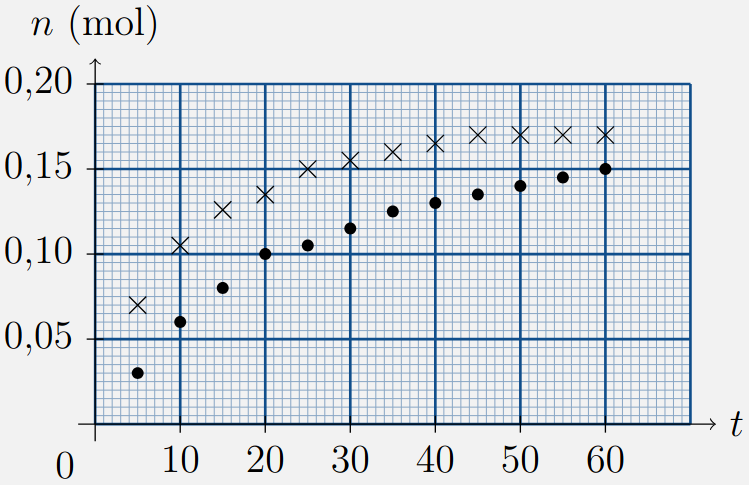
\includegraphics[width=0.9\linewidth]{swappy-20241230_104843.png}
\end{center}
\begin{enumerate}
    \item Quelle est la réaction chimique la plus rapide ?
    \item Pour chaque expérience, quelle est la vitesse d'apparition du composé (en mol.min$^{-1}$) à l'instant $t = 5$ min ? à $t = 60$ min ?
    \item On peut voir qu'au bout de $60$ min, la quantité de matière d'oxygène n'est pas la même dans les deux expériences. Expliquer.
\end{enumerate}
\end{exercice}

\end{multicols}

\end{document}
